% The original contents of this file and hello.tex are all comments and will be ignored during compilation.

% Input the examples on pages 8 to 10 of the task sheet to build up to the second deliverable of this task on page 11.
% Don't copy and paste from the PDF; this will add extraneous spaces and newlines.
% You should instead copy and paste from the source code of the task sheet (1.1 Hello, World!.tex) or retype the code.

% When you've completed the subtask at the end of page 11:
% - build the PDF (e.g. using the 'Recompile' button on Overleaf),
% - download the PDF (download icon is slightly to the right of 'Recompile')
%   - optionally, rename the PDF; by default, it will be named after this Overleaf project, but math.pdf might be a more appropriate name
% - download the .tex source code (click the three dots next to the selected filename in the left panel and then click 'Download', or copy and paste the contents to a blank file on your local filesystem).

% Now you can update the task status in Formatif to 'Ready for Feedback', and follow the prompts to upload 'hello.pdf', 'hello.tex', 'math.pdf' and 'math.tex' in that order.

\documentclass[12pt]{article}
\usepackage{amsmath} % for maths
\usepackage{algos-tasks}
\title{Typesetting Mathematics}
\author{Andre Monteiro}

\begin{document}
\maketitle

When describing algorithms, we often use compact sigma notation to describe repeated operations. For example, the operation
\begin{verbatim}
    sum = 0
    for i = 1 to n:
        sum = sum + A[i]
\end{verbatim}

would be written as $\displaystyle \sum_{i=1}^n A[i]$. In \LaTeX, this is written as
\begin{lstlisting}
\documentclass[12pt]{article}
\usepackage{amsmath} % for maths
\title{Typesetting Mathematics}
\author{Your name here}
\begin{document}
\maketitle
The following sigma notation represents a for loop that sums all the elements of an array $A$ of length $n$.
\[\sum_{i=1}^{n} A[i].\]
\end{lstlisting}

The \verb|\sum| command takes two arguments, \verb|lower| and \verb|upper| each enclosed in \verb|{...}| that define the lower and upper bound for the summation's range. However, where the elements are not ordered (i.e. a set), we should omit the \verb|upper| argument. For example,  \[ \sum_{e \in E} \operatorname{weight}(e) \] denotes the sum of all the edge weights in a graph (all edges $e \in E$).

Other tips you might want to be wary of: 
\begin{itemize}
    \item When quoting, be wary of orienting your inverted commas correctly. Using two inverted commas (\verb|'|) before and after a quote will output two inverted commas in the same direction. You should use a backtick (\verb|`|) to open a quote, and a regular inverted comma to close the quote.
    \item It's often good to have a cheat sheet ready for commonly used control structures. There are many available online, and it might be worth writing your own as you go along. If you're unsure what command gives a particular symbol, \href{https://detexify.kirelabs.org/classify.html}{Detexify} is an helpful tool available online.
    \begin{itemize}
        \item It's often worth asking staff about certain norms; say, usage of the \verb|\left| and \verb|\right| operators, and not using the asterisk for multiplication.
    \end{itemize}
\end{itemize}


\begin{question}
For this question, we want to practice using the \verb|\sum| command.
Copy the above snippet to \texttt{math.tex} and add the answers to the questions to \texttt{math.tex} in the \verb|enumerate| environment by using the \verb|\enumerate| command.
\begin{enumerate}
\item We want to write the expression 

\begin{center}
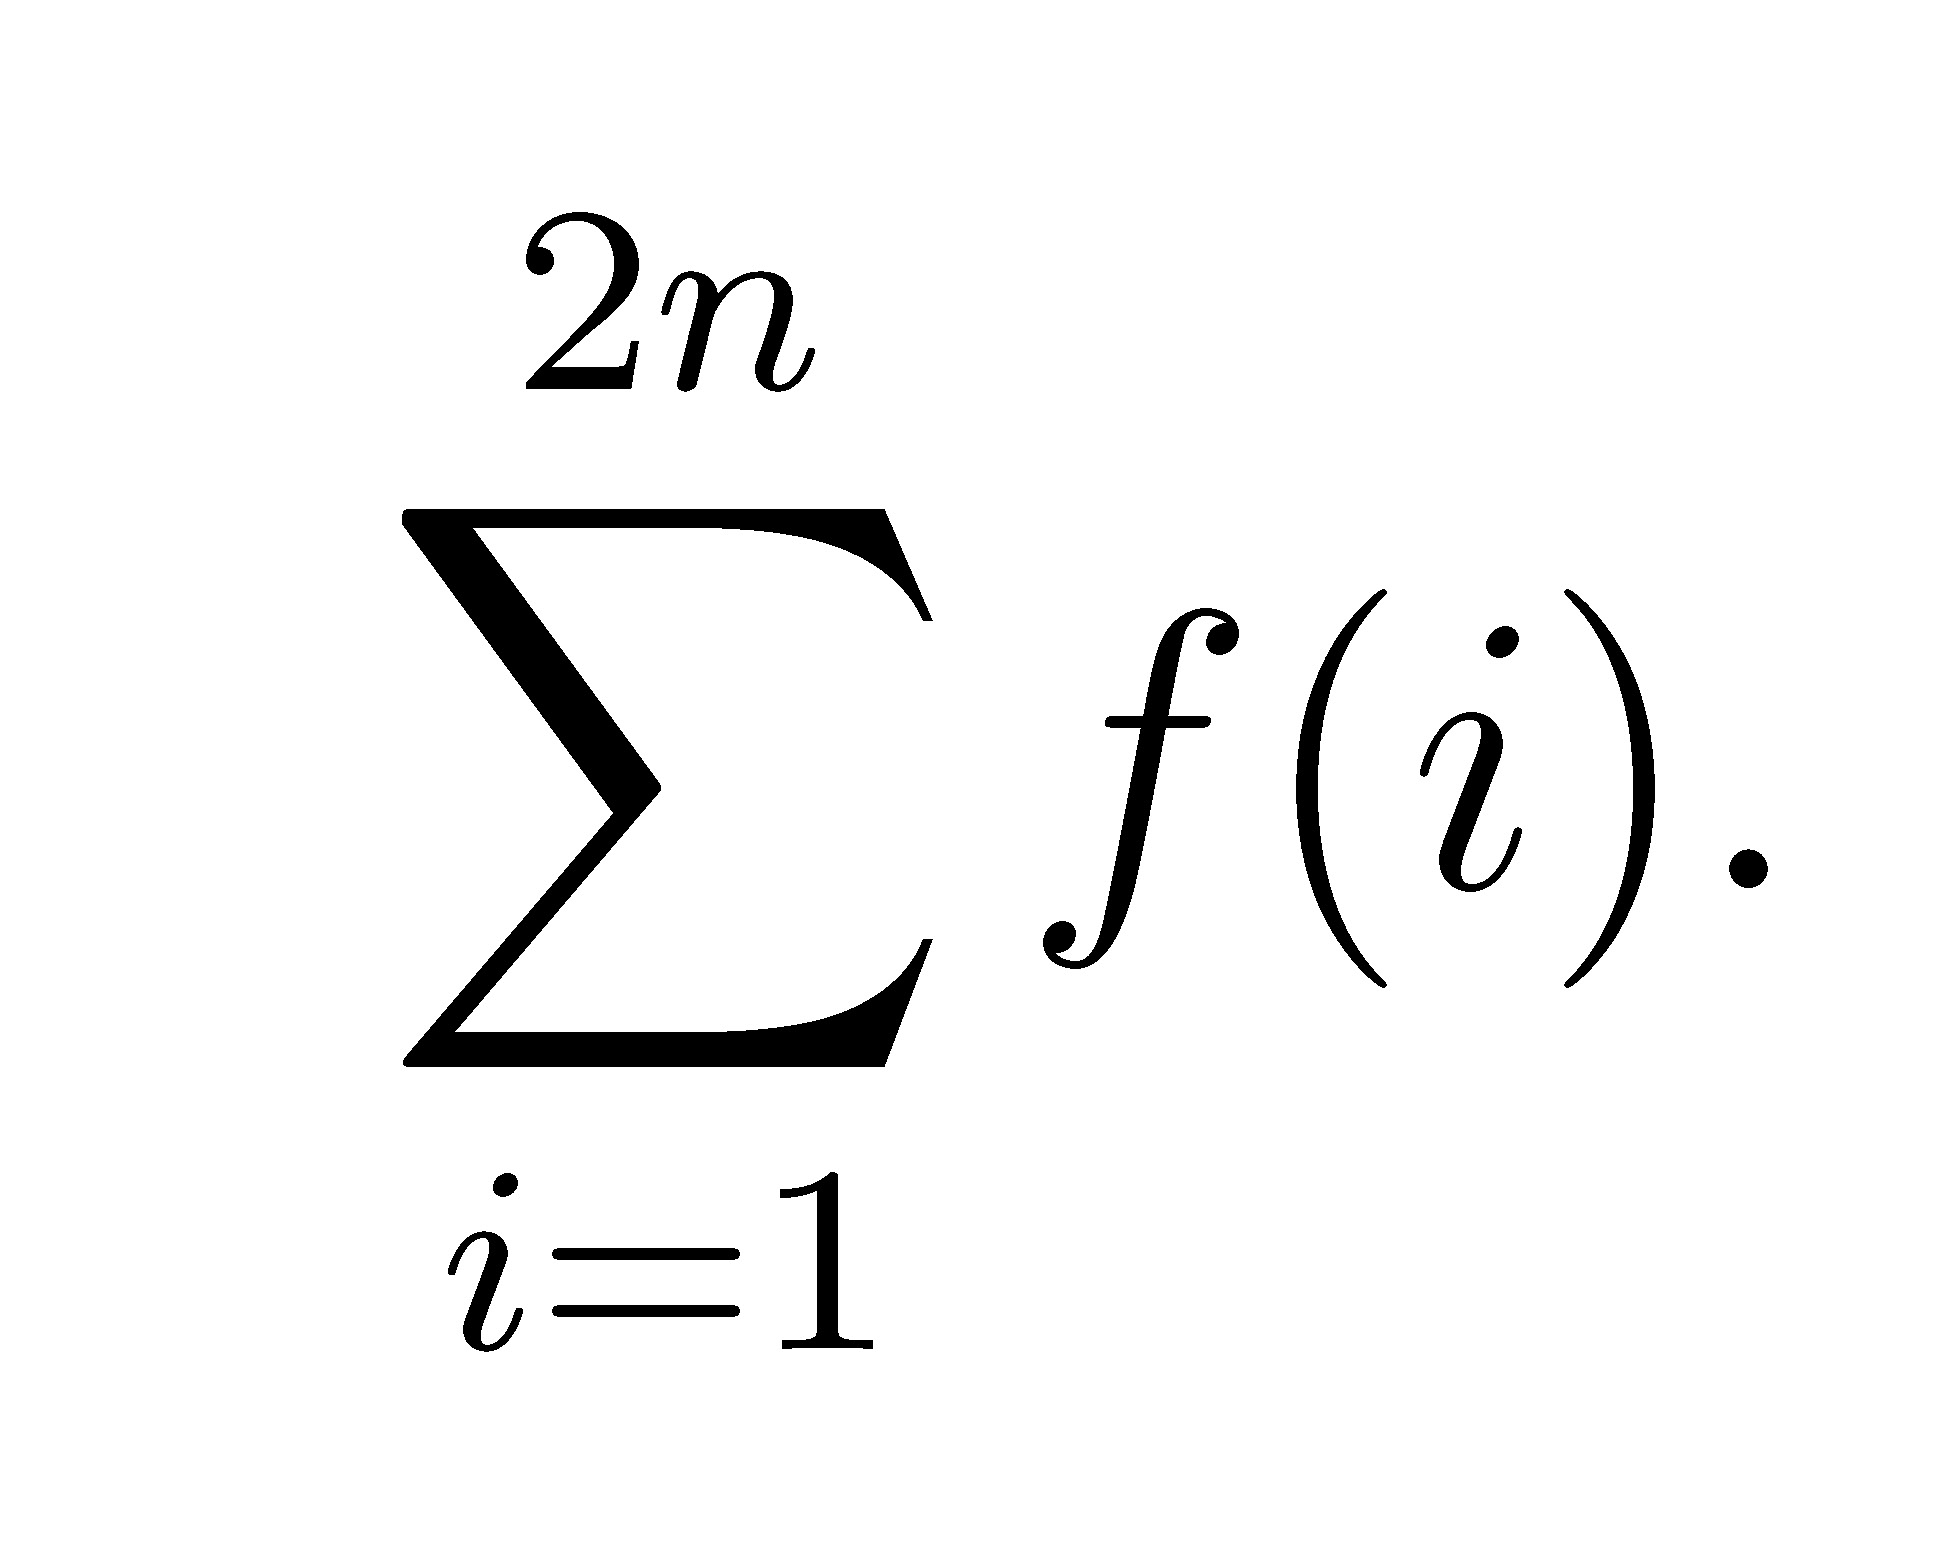
\includegraphics{eqn.jpg}
\end{center}
    We wrote the following \LaTeX\ code:
    \begin{center}
    \verb|\sum_i=1^2n f(i)|
    \end{center}
    What output does this produce? Identify and correct the errors in the code. \\
    \begin{enumerate}
        \item The following expression produces: \[\sum_i=1^2n f(i)\]
        Which is incorrect as it doesn't correctly encase the mathematical components in \verb|{}|.
        the correct \LaTeX code would be: \\
        \begin{center}
        \verb|\sum_{i=1}^{2n} f(i)| \\
        \end{center}
        Which evaluates to: 
        \begin{center}
        \[\sum_{i=1}^{2n} f(i).\] \\
        \end{center}
        \newpage
    \end{enumerate}
    \item Using sigma notation, write an expression for the total absolute difference between each pair of adjacent elements in an array $A$ of length $n$. For example, given the array $A = [1, 4, 2, 3]$, the total absolute difference is $\abs{1-4} + \abs{4-2} + \abs{2-3} = 6$.

    \textbf{Note:} \verb|\abs{...}| is not a control sequence defined in base \LaTeX\ or the maths packages, but rather a macro that we've defined in \texttt{algos-tasks.sty}. You can instead use \verb|\abs*{...}| for bars which scale with the height of the enclosed content.
    \begin{enumerate}
        \item The expression is: 
        \begin{center}
        \verb|\sum_{i=1}^{n-1} \abs*{A(i) - A(i+1)}\|
        \end{center}
        Which evaulates to: 
        \[\sum_{i=1}^{n-1}  \abs*{A(i) - A(i+1)}\]
    \end{enumerate}
\end{enumerate}

\textbf{Reminder:} Don't copy and paste from the PDF, as this will add extraneous spaces and newlines. You should instead copy and paste from the source code of the task sheet (\texttt{1.02 Hello, World!.tex}), or retype the code.
\end{question}
\end{document}
